\documentclass[14pt]{extbook}
\usepackage{multicol, enumerate, enumitem, hyperref, color, soul, setspace, parskip, fancyhdr} %General Packages
\usepackage{amssymb, amsthm, amsmath, bbm, latexsym, units, mathtools} %Math Packages
\everymath{\displaystyle} %All math in Display Style
% Packages with additional options
\usepackage[headsep=0.5cm,headheight=12pt, left=1 in,right= 1 in,top= 1 in,bottom= 1 in]{geometry}
\usepackage[usenames,dvipsnames]{xcolor}
\usepackage{dashrule}  % Package to use the command below to create lines between items
\newcommand{\litem}[1]{\item#1\hspace*{-1cm}\rule{\textwidth}{0.4pt}}
\pagestyle{fancy}
\lhead{Progress Quiz 5}
\chead{}
\rhead{Version C}
\lfoot{9912-2038}
\cfoot{}
\rfoot{Spring 2021}
\begin{document}

\begin{enumerate}
\litem{
Determine the domain of the function below.\[ f(x) = \frac{6}{15x^{2} +27 x + 12} \]\begin{enumerate}[label=\Alph*.]
\item \( \text{All Real numbers except } x = a \text{ and } x = b, \text{ where } a \in [-1.16, -0.98] \text{ and } b \in [-0.99, -0.75] \)
\item \( \text{All Real numbers except } x = a, \text{ where } a \in [-20.05, -19.94] \)
\item \( \text{All Real numbers.} \)
\item \( \text{All Real numbers except } x = a, \text{ where } a \in [-1.16, -0.98] \)
\item \( \text{All Real numbers except } x = a \text{ and } x = b, \text{ where } a \in [-20.05, -19.94] \text{ and } b \in [-9.06, -9] \)

\end{enumerate} }
\litem{
Choose the graph of the equation below.\[ f(x) = \frac{1}{x + 1} + 3 \]\begin{enumerate}[label=\Alph*.]
\begin{multicols}{2}\item 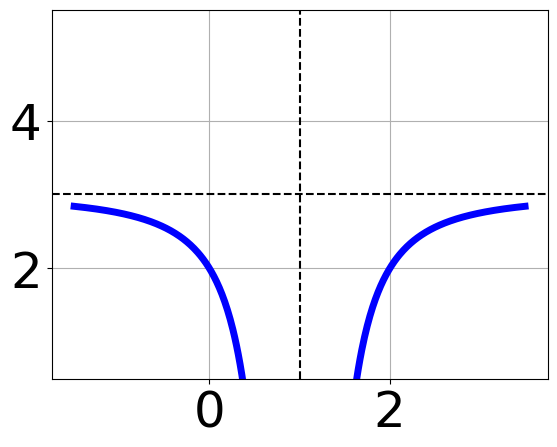
\includegraphics[width = 0.3\textwidth]{../Figures/rationalEquationToGraphCopyAC.png}\item 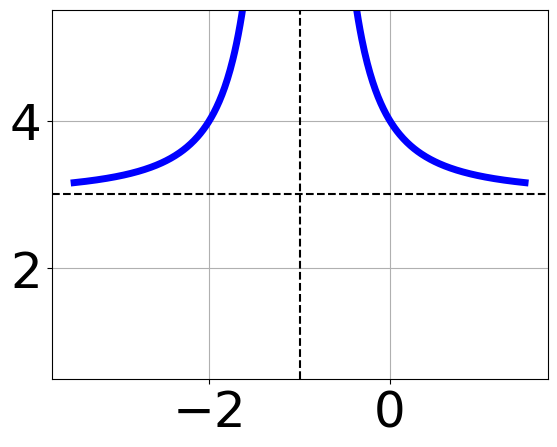
\includegraphics[width = 0.3\textwidth]{../Figures/rationalEquationToGraphCopyBC.png}\item 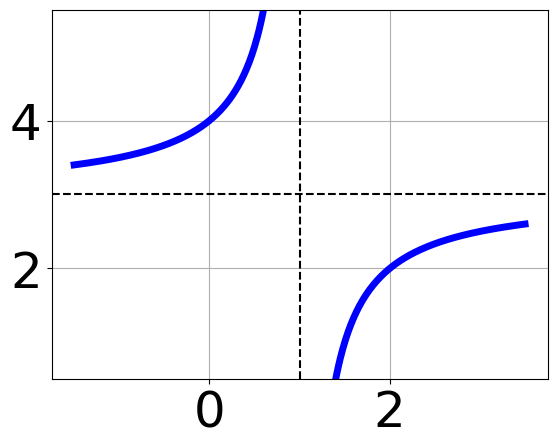
\includegraphics[width = 0.3\textwidth]{../Figures/rationalEquationToGraphCopyCC.png}\item 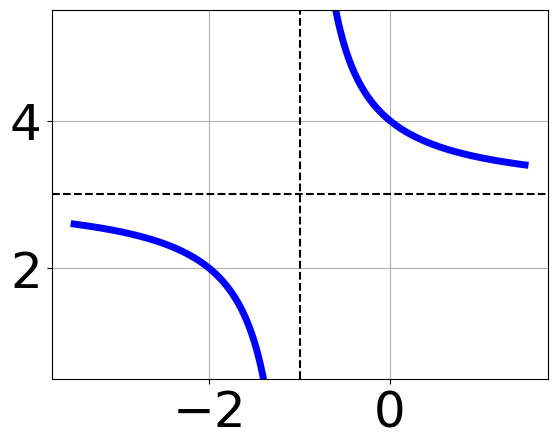
\includegraphics[width = 0.3\textwidth]{../Figures/rationalEquationToGraphCopyDC.png}\end{multicols}\item None of the above.
\end{enumerate} }
\litem{
Choose the equation of the function graphed below.
\begin{center}
    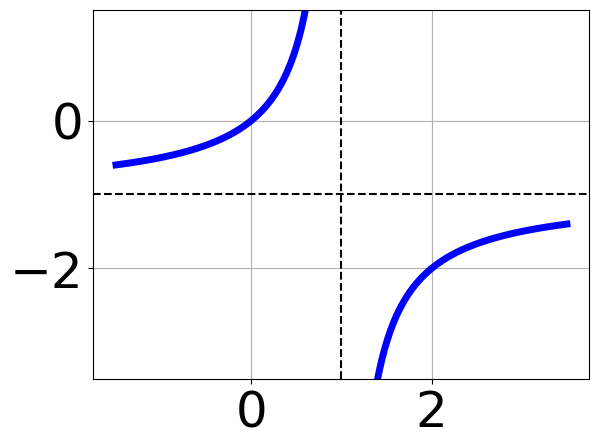
\includegraphics[width=0.5\textwidth]{../Figures/rationalGraphToEquationCopyC.png}
\end{center}
\begin{enumerate}[label=\Alph*.]
\item \( f(x) = \frac{1}{x + 1} + 3 \)
\item \( f(x) = \frac{-1}{x - 1} + 3 \)
\item \( f(x) = \frac{1}{(x + 1)^2} + 3 \)
\item \( f(x) = \frac{-1}{(x - 1)^2} + 3 \)
\item \( \text{None of the above} \)

\end{enumerate} }
\litem{
Choose the graph of the equation below.\[ f(x) = \frac{1}{(x - 2)^2} + 2 \]\begin{enumerate}[label=\Alph*.]
\begin{multicols}{2}\item 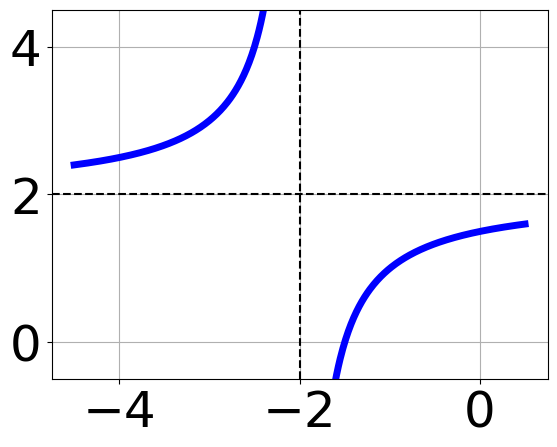
\includegraphics[width = 0.3\textwidth]{../Figures/rationalEquationToGraphAC.png}\item 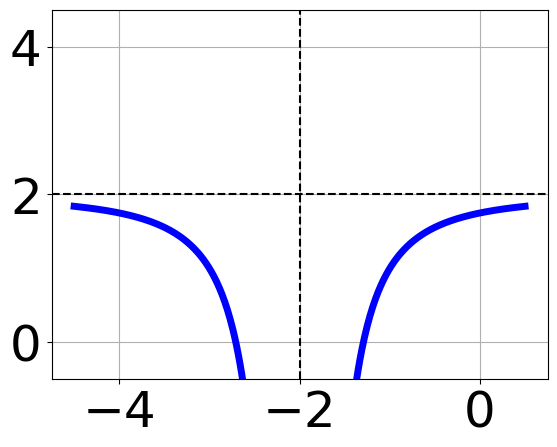
\includegraphics[width = 0.3\textwidth]{../Figures/rationalEquationToGraphBC.png}\item 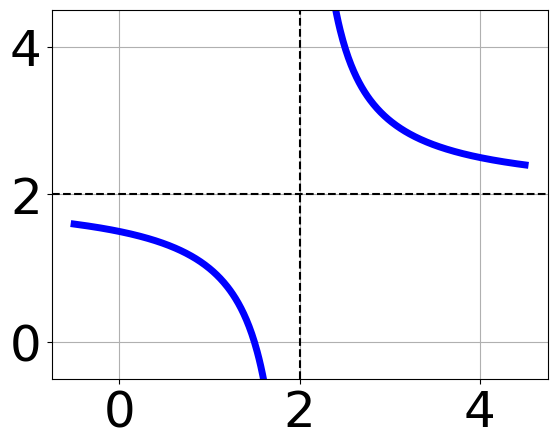
\includegraphics[width = 0.3\textwidth]{../Figures/rationalEquationToGraphCC.png}\item 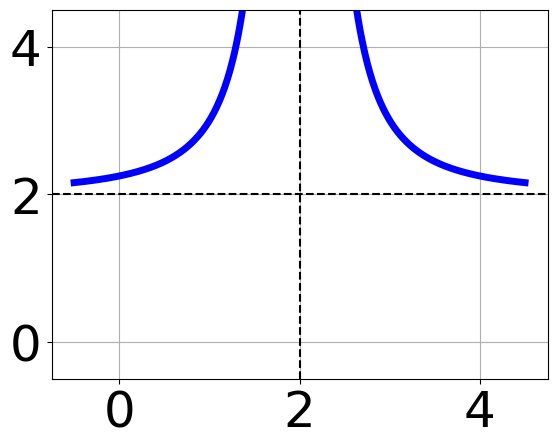
\includegraphics[width = 0.3\textwidth]{../Figures/rationalEquationToGraphDC.png}\end{multicols}\item None of the above.
\end{enumerate} }
\litem{
Solve the rational equation below. Then, choose the interval(s) that the solution(s) belongs to.\[ \frac{88}{44x -22} + 1 = \frac{88}{44x -22} \]\begin{enumerate}[label=\Alph*.]
\item \( x \in [-1.3,-0.4] \)
\item \( x_1 \in [-1.3, -0.4] \text{ and } x_2 \in [0.5,1.5] \)
\item \( x \in [0.5,1.5] \)
\item \( \text{All solutions lead to invalid or complex values in the equation.} \)
\item \( x_1 \in [0.3, 1.5] \text{ and } x_2 \in [0.5,1.5] \)

\end{enumerate} }
\litem{
Solve the rational equation below. Then, choose the interval(s) that the solution(s) belongs to.\[ \frac{-6x}{-7x -7} + \frac{-2x^{2}}{14x^{2} +49 x + 35} = \frac{-3}{-2x -5} \]\begin{enumerate}[label=\Alph*.]
\item \( x_1 \in [0.96, 1.29] \text{ and } x_2 \in [-3.59,-1.43] \)
\item \( \text{All solutions lead to invalid or complex values in the equation.} \)
\item \( x_1 \in [0.96, 1.29] \text{ and } x_2 \in [-1.5,-0.92] \)
\item \( x \in [-3.1,-2.03] \)
\item \( x \in [-2.28,-1.93] \)

\end{enumerate} }
\litem{
Determine the domain of the function below.\[ f(x) = \frac{5}{24x^{2} -14 x -20} \]\begin{enumerate}[label=\Alph*.]
\item \( \text{All Real numbers except } x = a \text{ and } x = b, \text{ where } a \in [-1.9, -0.1] \text{ and } b \in [0.6, 2.8] \)
\item \( \text{All Real numbers except } x = a \text{ and } x = b, \text{ where } a \in [-25.1, -23.2] \text{ and } b \in [19.1, 20.6] \)
\item \( \text{All Real numbers except } x = a, \text{ where } a \in [-25.1, -23.2] \)
\item \( \text{All Real numbers except } x = a, \text{ where } a \in [-1.9, -0.1] \)
\item \( \text{All Real numbers.} \)

\end{enumerate} }
\litem{
Solve the rational equation below. Then, choose the interval(s) that the solution(s) belongs to.\[ \frac{3}{3x -2} + 6 = \frac{-2}{27x -18} \]\begin{enumerate}[label=\Alph*.]
\item \( \text{All solutions lead to invalid or complex values in the equation.} \)
\item \( x_1 \in [0.26, 0.47] \text{ and } x_2 \in [-0.51,3.49] \)
\item \( x \in [-0.89,-0.84] \)
\item \( x \in [0.49,2.49] \)
\item \( x_1 \in [-0.89, -0.84] \text{ and } x_2 \in [-0.51,3.49] \)

\end{enumerate} }
\litem{
Solve the rational equation below. Then, choose the interval(s) that the solution(s) belongs to.\[ \frac{-4x}{5x -5} + \frac{-7x^{2}}{-35x^{2} + 35} = \frac{-5}{-7x -7} \]\begin{enumerate}[label=\Alph*.]
\item \( x \in [-2.4,-0.1] \)
\item \( \text{All solutions lead to invalid or complex values in the equation.} \)
\item \( x_1 \in [-0.4, 0.7] \text{ and } x_2 \in [-6.93,-0.93] \)
\item \( x_1 \in [-0.4, 0.7] \text{ and } x_2 \in [0,11] \)
\item \( x \in [-5.1,-1.5] \)

\end{enumerate} }
\litem{
Choose the equation of the function graphed below.
\begin{center}
    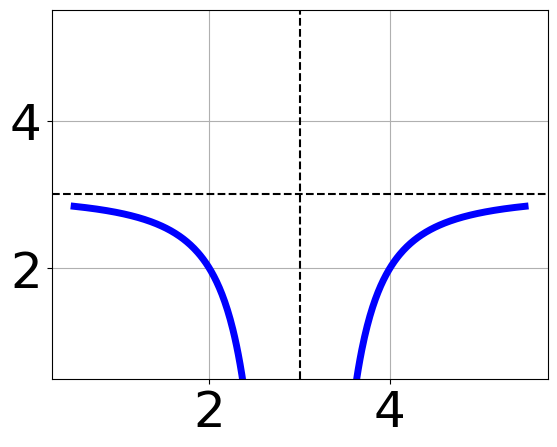
\includegraphics[width=0.5\textwidth]{../Figures/rationalGraphToEquationC.png}
\end{center}
\begin{enumerate}[label=\Alph*.]
\item \( f(x) = \frac{-1}{x + 3} + 1 \)
\item \( f(x) = \frac{1}{x - 3} + 1 \)
\item \( f(x) = \frac{1}{(x - 3)^2} + 1 \)
\item \( f(x) = \frac{-1}{(x + 3)^2} + 1 \)
\item \( \text{None of the above} \)

\end{enumerate} }
\end{enumerate}

\end{document}